\documentclass[12pt, a4paperm, twoside]{report}

\usepackage[cyr]{aeguill}
\usepackage[pdftex]{graphicx}
\usepackage[pdftex]{thumbpdf}
\DeclareGraphicsExtensions{.jpg,.pdf,.png,.gif,.ps,.pdf,.eps}
\usepackage[pdftex,colorlinks=true,linkcolor=blue,citecolor=blue,urlcolor=blue]{hyperref}
\usepackage{internship}
\usepackage{enumerate}
\usepackage{array}
\usepackage{eurosym}
\usepackage{makeidx}
\usepackage{glosstex}
\usepackage[numbers]{natbib}
%\usepackage{listing}
\usepackage{verbatim}
%\lstset{frame=single}
%\lstset{basicstyle=\small}
%\lstset{extendedchars=true,inputencoding=UTF8}
%\lstset{breaklines=true}
%\lstset{float=tbph}
\usepackage{a4wide}
\RequirePackage{fancyhdr}
\fancyfoot{}
\pagestyle{fancy}

\makeindex
% glossary
\makeglossary
% figure path
%\graphicspath{{Pix/}}


\title{Internship}
\subtitle{Report}
\author{Eric Keller}
\email{keller\_e@epita.fr}
\date{\today}
\location{Bonaduz}
\blurb{ blah }
\uid{GISTR}
\subject{Test Process for a medical Ventilator}
\tutor{Roger Altermatt}
\logo{img/Logo_company.jpg}
\school{epita.jpg}
\compagny{HAMILTON MEDICAL AG \\Via Nova \\CH-7403 Rhaezuens/Switzerland}

\begin{document}
%\doparttoc
\maketitle
\newpage
\tableofcontents
\listoffigures
\thispagestyle{empty}
\pagenumbering{arabic}
\newpage
% summary of the internship_____________________________________________________ 2 pages
\abstract{

For my last year internship, I choose the \emph{Hamilton-Medical} company located in Bonaduz, Switzerland.
\emph{Hamilton-Medical} is part of the \emph{Hamilton} group, founded in Reno USA in 1956 by Clark Hamilton.
In 1983 Hamilton-Medical AG was born form the \emph{Respirator} Project.
Today \emph{Hamilton-Medical} has the 4th worldwide market position.
\\
\\
I joined the \emph{New Products} division, and worked in a team of 15 people, on a Clinical Respirator, named Nemo.
The Product was already started for more than one year, I arrived on a stage where parts of the basic functionality were coded.
Yet the test process was not exiting, the project should be launched on April 2008. A lot of work is planned, for the intermediate 0.5 version, which should be ready for clinical test in Chur \emph{Kantonspital} on 20th of August.
\\
\\
My work consist in the one hand conceiving the test concept (adaptation of the current workflow), on the other hand, building the tests cases for the project. Only two people are dedicated to do all these tasks, Ulrich Hauser and I. Knowing that all literature explains that critical software development require as much time for the developing phase as for the testing phase. In such a short time we have to test the whole project as efficiently as we can, this is a challenging work.
\\
\\
The Nemo project is coded in C++ on a Power PC architecture, with a WindRiver VxWorks Operating system. This project is the first to use the Object Oriented technology. The main tool used for develop the project is Telelogic Rhapsody, a UML modler. The developper design the software as UML diagram, integrate the code functionalities, generate the C++ code and compile it for VxWorks.
\\
This process brings some transparency from modelisation to code, and gives a direct link between UML design and code, it also gain development time.
\\
\\
I was quickly accepted among the development team, after 2 month of internship a first positiv meeting with my supervisor, ended up to a proposition of beeing hired. I earn a valuable experience of this internship, working in medical environment gives me another look to project conception, human life are part of the game, so we have to develop a high quality/reliable product.
\\
\\
This internship report aims to present my work at the R\&D section of \emph{Hamilton-Medical}, during the past 5 month.
}

\newpage
%----------------------------------------------------------------------------------------------------------------------------------------------------------

\chapter{Introduction}%________________________________________________________ 10 pages
% this section should help the jury to understand your internship complexity.
My internship in \emph{Hamilton-Medical}, was challenging at all point of view. From the foreign German language to the efficient work I had to furnish.
In the following section I will present you the initial internship objectives and the changes in the subject. I will also introduce the background of the company, explaining how long it is working in this business. Finally I will describe of the context in which I worked.

\section{Initial internship subject and its objectives}%___________________________________ 15 lines
%internship subject exposing the aims
Originally, the internship subject was\index{Objective}:
\\
\textbf{Test the Nemo Project, a clinical respirator, against its technical specifications}
\\
\\
The primary objective of the internship was to get a tested and stable version of the software. Another objective is to test the complete (software and hardware) project on patient in a clinical environment, on 20th August.
\\
There were different test to run on the software which is more than 70 000 lines of code spread among hundred of classes:
\begin{itemize}
\item Test the code of critical modules.
\item Test the Rhapsody framework generated code (especially the state charts diagrams).
\item Test the GUI.
\item Test the whole system, software with the final hardware.
\item Test the project for memory leaks.
\end{itemize}

\section{Explanation of changes in subject} \index{Internship changes}
%some details about internship changes in subjects
As the given subject was wide, some changes/precisions were operated in the subject, but the main goal remains the same. Before I could begin the testing phase of the project, I had to pick up a test tool  among the existing one. I also elaborate the test concept with Ulrich Hauser, who arrived one month after me.
\\
This means that no test workflow was available, and we\footnote{Ulrich and I} had to modify the actual development workflow to include the testing and bug report phase.
I closely worked with the G5\footnote{G5 is the new product launched on May 2007} development and testing team. I was explained the test process they used.
\\
The second change in the subject was that I should write a \emph{cook book} about the test tool we were using. So the developers team could also test the software.

\section{Company Business}%____________________________________________________________ 3 pages
%concurrence of the company, HM perspectives, situation of my internship among the company.

\subsection{The Hamilton group}

\subsubsection{Hamilton history} \index{Hamilton history}
The history of the company \emph{Hamilton}, was started by a pioneering invention that Clark Hamilton made in 1947 in his garage. The Microliter syringe with the product number 701 was the foundation for an internationally operating company. In 1955, the success of \emph{Hamilton}'s products is enormous, Hamilton Co., US, is founded in Reno.
\\
In 1966, \emph{Hamilton}'s production facilities start to operate worldwide, HAMILTON BONADUZ AG Hamilton. The creation of the R\&D in Bonaduz in 1974 was the logic following. Finally the Liquid Handling Robots and OEM Business started in 1977.

\subsubsection{Hamilton Sectors}

Today the Microliter syringe is a firmly established element in the work of researchers all over the world. Clark Hamilton's syringe permitted the dosing of liquids with considerably great precision, despite its leadership in this sector, \emph{Hamilton} continues to expend its research to other sector:
\\
\begin{itemize}
\item \emph{robotics} the robotics business unit develops, produces and markets fully automated pipetting and analysis systems for routine use in research and diagnostic laboratories all over the world.
\item \emph{liquid handling} \emph{Hamilton} is the undisputed global market leader in this segment thanks to the invention of the Microliter syringe. The company's legendary precision in the dosing of liquids supports analyses in a very broad field of application.
\item \emph{analytic} among scientists, the sensors and calibration solutions of \emph{Hamilton} are regarded as being particularly precise. The extremely precise sensors are used in pH measurements and in the measurement of oxygen and conductivity.
\item \emph{medical} \emph{Hamilton-Medical}, an independent joint stock company with a strong operational link to \emph{Hamilton} in Bonaduz, is specialised in ventilator systems and their accessories. The company's products are used in intensive care units, recovery rooms and nursing homes.
\end{itemize}

\emph{Hamilton-Medical} is a member of the \emph{Hamilton} Group, a privately owned company that now employs approximately 1,000 people. Bonaduz is the major pole of production employing more than 400 people.

\subsection{The Hamilton-Medical AG}
Based in Switzerland, it combines the quality of Swiss manufacturing systems with global resources and the reliability of a focused organization.
Being the specialist in \emph{Intelligent Ventilation}, it is perfectly positioned to respond to all demands, now and in the future.
\\
\subsubsection{History} \index{Hamilton-Medical history}
In 1981, Dr. Amadeus Meier started the 'Respirator' Project, two years later, \emph{Hamilton-Medical AG} was formed in Rhaezuenz Swizerland. In 1984, HAMILTON MEDICAL sells its first ventilator to the Kantonspital Chur, Switzerland.
\\
\\
\emph{Hamilton-Medical} mission is to provide care with safe and reliable respiratory therapy devices through development, manufacturing, and distribution of innovative products and services, for ventilated patients in hospitals and sub acute care facilities, worldwide.
\\
\\
The core competencies are:
\\
\begin{itemize}
\item High-precision gas valves for medical applications
\item Sensor technology for respiratory gases
\item Lung function analysis and Graphical User Interface
\item Automation of respiratory support devices
\end{itemize}

\subsubsection{Hamilton-Medical products} \index{products}
\emph{Hamilton-Medical} has a large range of products adapted to different situations:

\begin{description}
\item [Anabela] The ARABELLA is an easy to operate system proven to effectively and safely deliver NCPAP\footnote{Nasal Continuous positive airway pressure} therapy. The noninvasive Universal Generator and Prongs reduce the work of breathing while maintaining a stable NCPAP level throughout the respiratory cycle for greater comfort for your very small patients. When used in conjunction with early extubation and NCPAP first strategies, the ARABELLA minimizes the need for intubation and mechanical ventilation.
\item [Raphael] RAPHAEL ventilators feature a compact, biphasic design that helps patients to breathe more freely in all modes and phases. Small enough to fit into almost any ICU environment, and competitively priced, they cover the full range of clinical requirements: invasive ventilation, automated ventilation with Adaptive Support Ventilation (ASV), and Non-Invasive Ventilation (NIV).
\item [Galileo] The GALILEO ventilator family offers a full spectrum of capabilities, including invasive to noninvasive and advanced ventilation modes, plus tube resistance compensation. Intelligent features like adaptive support ventilation (ASV) and the P/V Tool help you determine appropriate ventilator settings, based on the patient's respiratory mechanics.
\item [G5] The HAMILTON-G5 is the first ventilator to provide, a new Ventilation Cockpit that is designed to improve safety through intuitive operation and monitoring; proven closed-loop ventilation that automatically applies lung-protective strategies, reduces the risk of operator error, and promotes early weaning. The HAMILTON-G5 was designed to provide Intelligent Ventilation, delivering
\begin{itemize}
\item superior performance in complex environments
\item improved patient outcomes
\item reduced costs
\end{itemize}
\end{description}


\begin{figure}[ht]
\centering
  \framebox{
    \begin{minipage}{5cm}
     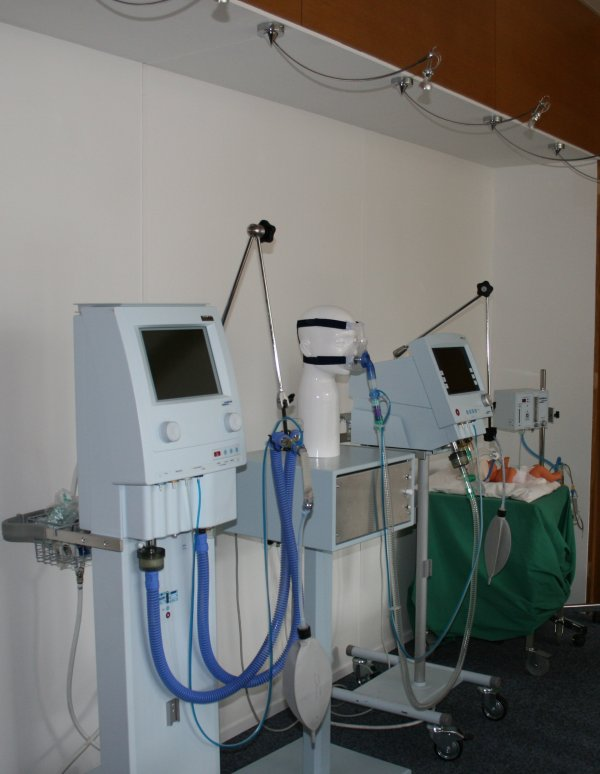
\includegraphics[width=\textwidth]{img/respirators.jpg}
    \end{minipage}}
 \caption{\label{Hamilton-Medical Respirator}
Hamilton-Medical Respirator}
\end{figure}


\begin{figure}[ht]
\centering
  \framebox{
    \begin{minipage}{5cm}
     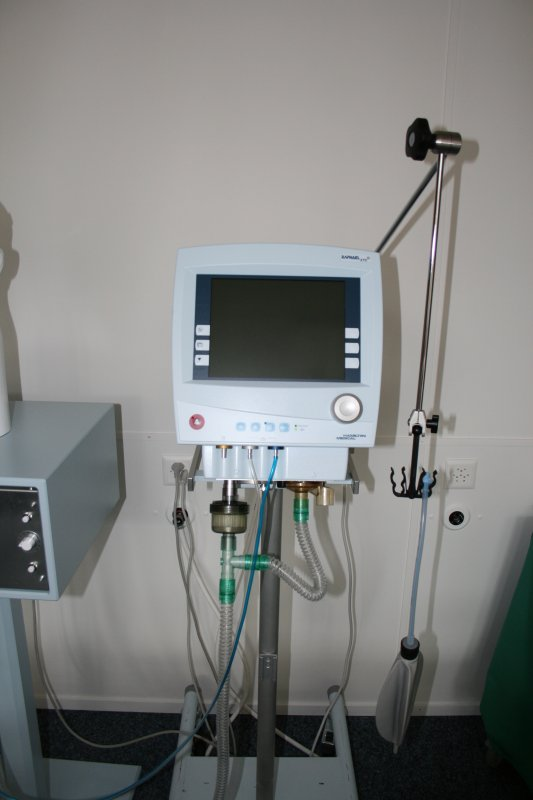
\includegraphics[width=\textwidth]{img/beatmungsgeraet.jpg}
    \end{minipage}}
 \caption{\label{Hamilton-Medical Respirator}
Hamilton-Medical Respirator}
\end{figure}

\section{Competitors} \index{competitors}
Several competitors are developing respirator for the ICU\footnote{Intensive Care Unit}:
\\
\begin{itemize}
\item Draeger
\item Maquet (Siemens)
\item Tyco
\item Viasys
\item eVent Medical
\item Versamed
\item Taema
\item Saime
\end{itemize}

\begin{figure} [ht]
\centering
  \framebox{
    \begin{minipage}{14cm}
     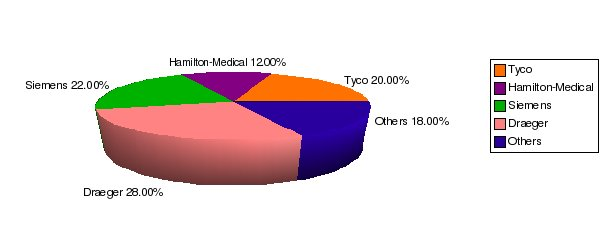
\includegraphics[width=\textwidth]{img/marketShare2.jpg}
    \end{minipage}}
 \caption{\label{Intensive Care ventilator market share}
 Intensive Care ventilator market share}
\end{figure}

Tyco a subsidiary company of Puritan Bennett, has been a leading innovator of medical ventilation and respiratory care devices for over 50 years.
\\
Worldwide MAQUET ranks among the leading providers of medical technology products and services for Operating Rooms and Intensive Care Units.
\\
First seen as a research company, \emph{Hamilton-Medical} emerged in 2003 as the fourth largest ventilator company in the world.

\section{Perspectives}
Based on demographic and socio-cultural changes, new economic challenges, Hamilton-Medical AG aims to be one of the main actors on the respirator market.
\\
On average:
\begin{itemize}
\item everyone will be in intensive care once in their life (some never, some several times).
\item 50\% of us will spend time in the ICU in the last year of live.
\item 20\% of us will die in an ICU.
\end{itemize}

Since the industrialized world gets older, the Intensive Care beds are increasing it those developed countries and the Chronic Obstructive Pulmonary Disease becomes a major health problem.
\\
Plus the health care system is a major cost factor, as health expenditures are even growing faster.
\\
This contributes all to create new challenges and opportunities in Intensive Care. Some solutions are in sight:
\begin{itemize}
\item Quality of life will replace survival as primary criteria
\item Prognostic scores will be improved
\item Data management systems will be used to support decisions
\item Cost-value ratios will gain influence on therapy and preventive measures
\item Genetic therapy will gain influence
\item Robotics will support nursing
\item ICUs will build supra-regional networks
\end{itemize}

\emph{Hamilton-Medical} is dedicated to become thought leader in ventilation, thanks to the most innovative products with lowest cost of ownership.

\section{The Company knowledge about my internship subject}
% company know how about the subject, in relation with the global aim of the company, relation with my supervisor during the internship
% project G5 know how, test know how, Urs Reidt, UT know How Christian Frehner
\emph{Hamilton-Medical} has more than 20 years of experience, in the development of Intensive Care Products. They market worldwide, meaning \emph{Hamilton-Medical} products have to fit to international Norms\footnote{the FDA (Food and Drogue Administration), and European Medical Norm are the most popular}.
\\
The company was aware about my objectives and the difficulty of the testing process. With the previous projects they have acquired a good knowledge of software testing. The Test Tool they are use to employ have done their proof, in the industry world, the R\&D manager is also open to adopt new method if it can lead to effective work.
\\
Unfortunately their is no written trace about how to test a Hamilton-Medical Product, but thanks to some competent people of the G5 project, I was explained how they proceed.
\\
Roger Altermatt my direct internship supervisor, has a strong know how about Hardware, but the relevant software testing question were discussed with the headmaster of the R\&D section Urs Reidt, Software engineer.

\section{My knowledge about the internship subject}
% intern knowhow about the subject detail why this internship is fitting to the GISTR Attitude, Motivation about this intership.
Testing the embedded software of a \emph{Hamilton-Medical} device, is a challenging task. This domain was not discussed during my EPITA studies. Well for most of the ING 1 Project we had to furnish a large amount of test cases, but this testing technique are a little part of Software testing.
\\
We never were explained how we should test a software, I mean it goes parallel with the software development. Testing a software aim is not to verify the software behaviour, but find errors and prove that the software do what is not supposed to be done.
\\
This internship has given me an opportunity to extend my knowledge about Testing, from choosing the test tools, to establishing a Test concept, and creating relevant test cases.
\\ %TODO reference to the art of software testing.
I have read a few books about Software testing, and especially about Object oriented Testing. I also assisted to some web seminar proposed by Telelogic\footnote{how Telelogic Rhapsody achieves object oriented testing}.

% temporary newpage
%\newpage
\section{Detailed working context}
%working context, means furnished by the company, access to the documentation, awareness of the competent people, the goal is to describe what I used to achieve efficiently my internship subject.
% VxWorks course in Munich unit Tester workshop in da house, framework workshop in da house, Design walkthrough.

\emph{Hamilton-Medical} supplied me a bi-monitor Desktop computer, working under Microsoft Windows operating system. I have the administrator rights and authorisation to install all the software I need for achieve my work.
\\
\\
The second week of my internship I obtained a Licence for the WindRiver Framework tools: Industrial devices 3.3. I explored its possibilities creating some dummy project, working on the Power PC simulator. I also granded the access to the Nemo documentation, trough an intern software, EDO\footnote{EDO is a document manager using PVCS (Polytron Version Control System)}. I had access to numerous WindRiver hardcopy books, and Nemo intern Documents, technical specification...
\\
\\
The development is insured by Rhapsody, which I also got a licence, allowing me to explore the project trough UML diagrams. On February I received a Nemo target prototype, composed of the main board and touch-screen. Accessing to the Nemo source code, I could operate the first build of the project.
\\
\\
Trough the intranet I could access to all the organisation and quality management documentation, an intern telephone book is also available. Various photocopier permit me to print documentation, a copy centre give the possibility to print a larger documentation such as user reference...
\\
\\
At the end of February, I assisted to a one week WindRiver workshop in Munich, which completed the EPITA introduction lesson. On March we organised a Unit Tester workshop at Hamilton Medical explaining how the IPL test tool works. Finally I participate to the Rhapsody framework course.

\newpage
%----------------------------------------------------------------------------------------------------------------------------------------------------------
% parler de fit for life
\chapter{Company organisation}%_____________________________________________________________________________ 25 pages
% in this section, the jury will understand the human and organisation relations in which the internship was done, measure its complexity, and measure my adaptation
\index{organisation}
The \emph{Hamilton} is a family owned enterprise, the leader of a board of directors for Hamilton Bonaduz is Dan Hamilton, the Chief Executive Officer is Andreas Wieland for the last ten years, also chairman of the board for Hamilton-Medical. The company organisation is assumed to be pyramidal, since all the sectors of activity have there own CEO.
\\
The Human resources are available for both \emph{Hamilton Bonaduz} and \emph{Hamilton-Medical} company. Their main activity is to ensure the wellness of the employee. For accomplishing this objective, a trimester 'Fit For Life' program is available. We could take part to numerous activities, fitness studio, mountain bike technique, running technique, cooking course, ...

\begin{figure}[h]
\centering
  \framebox{
    \begin{minipage}{10cm}
     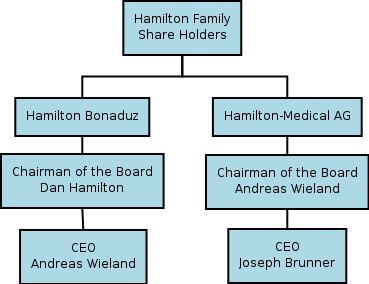
\includegraphics[width=\textwidth]{img/Hamilton-Organisation.jpg}
    \end{minipage}}
 \caption{\label{Hamilton Bonaduz Organisation}
Hamilton Bonaduz Organisation}
\end{figure}

Joseph Brunner is the \emph{Hamilton-Medical}'s CEO, the organisation among the \emph{Hamilton-Medical} branch is distributed in this matrix organisation:
\index{organisation}
\begin{itemize}
\item New Products
\item Sales
\item Marketing
\item Training
\end{itemize}

\begin{figure}[h]
\centering
  \framebox{
    \begin{minipage}{12cm}
     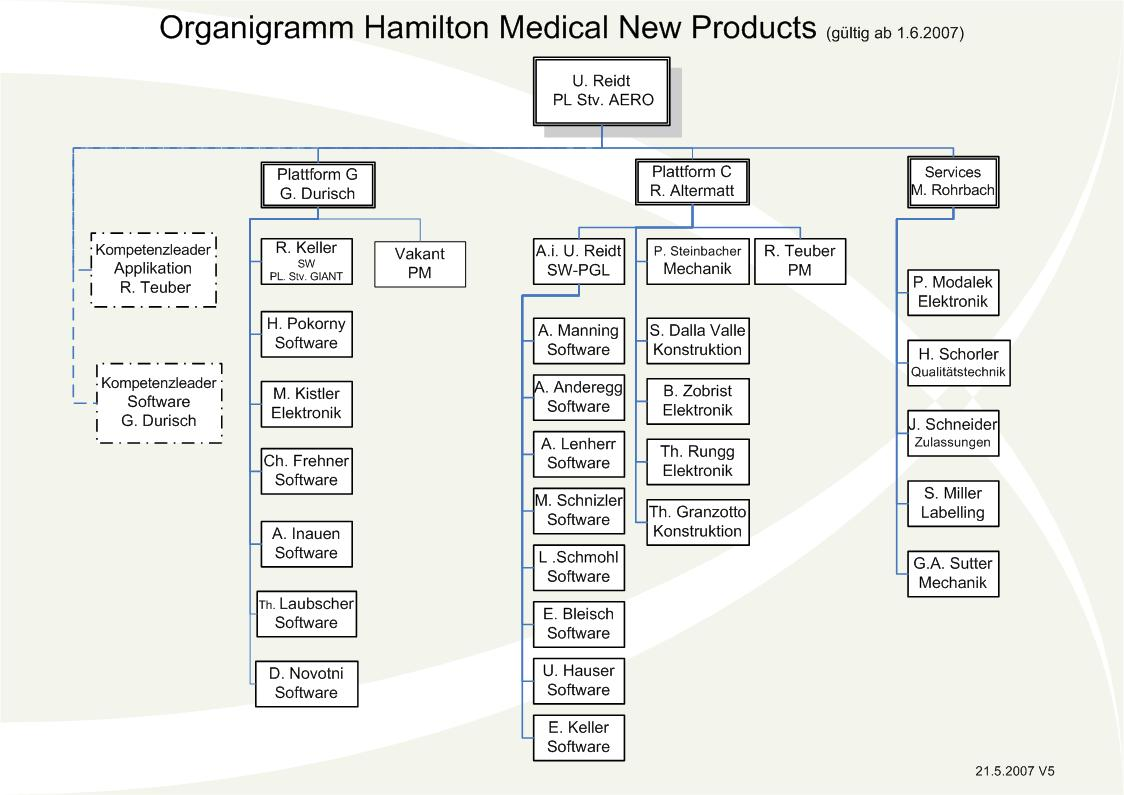
\includegraphics[width=\textwidth]{img/organisation-Medical.jpg}
    \end{minipage}}
 \caption{\label{Hamilton Medical organisation}
Hamilton-Medical organisation}
\end{figure}

I joined the Nemo Project development team, supervised by Roger Altermatt. The team can be split in four domains, Hardware/Electronic, Software, Constructor, Tester:

%\begin{figure}[hp]
%\centering
%  \framebox{
%    \begin{minipage}{12cm}
%     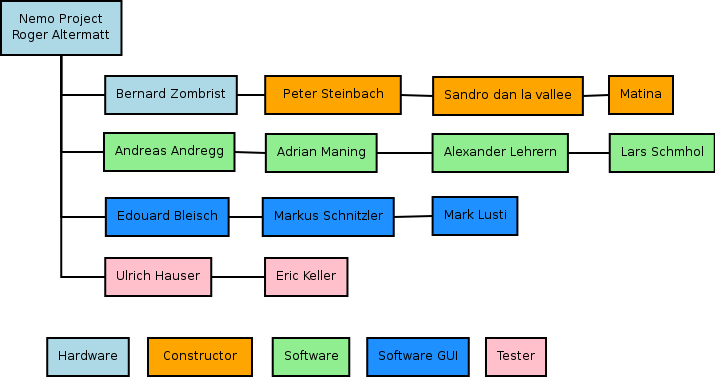
\includegraphics[width=\textwidth]{img/Nemo-organisation.png}
%    \end{minipage}}
% \caption{\label{Nemo Project organisation}
%Nemo Project organisation}
%\end{figure}

\begin{description}
\item [Hardware] the Power PC main board design had to be adapted to the project needs, so several sensors were integrated, as well as the pneumatic valve controller, USB port, hard keys ...
\item [Software] in one hand all the visual aspect of the software product is developed, GUI, real time curve, service software(auto diagnostic and calibration of the sensor). In the other hand the heart of the software, as the alarming, gas delivery, breath generator, are developed in parallel.
\item [Constructor] The Nemo project was design to integer a blower delivering a stable precision. Such parts were developed internally by the Constructor team.
\item [Tester] first establishing the Test concept, the Tester team, upgraded the current workflow intergrating the Testing and Tracking workflow. Finally the creation of the software test cases.
\end{description}


% description du projet dans sa globalite, parler de la version 0.5
\section{Project time-line}
% mentioning the steps and document I realised and their place in the project goal. If possible the step validating going from one to another step. mention the step serially or parallel, also mention the quality process.

On my arrival to \emph{Hamilton-Medical} I was briefed on the project software modelisation, hardware, and pneumatics. I had a lot of intern documentation, about the Nemo project, to read during my first weeks.
\\
The first objective of my internship was to acquire a solid know how about software testing. I had to perform research on both testing software world, being general but also more specific about software testing in embedded object oriented language. In parallel, I explored the possibility of using some Linux Based computer to ease the automation of the testing task. In fact using Windows command interpreter was simply not adapted in comparison of script shell or Perl scripting.
\\
As the Nemo software team was developing it software under Windows XP, I could try to install WindRiver Industrial Device under a Linux Operating system, compile some WindRiver project, and finally explain that the whole automation process was easier to handle under Linux, from the readability of scripts to the extended possibilities given by Linux.
\\
I established a meeting with Christian Frehner, one of the responsible of G5 Project software testing. He explained me, after exposing me the evolution of the test tools, how they test their entire software, from functionalities to GUI. My next objective was to analyse how they process to find a good way to adapt it to the Nemo project.
\\
\\
After a Software meeting with my supervisor, I got my next commitment, which consist in writing an intern document, concerning the available test tools. So I first evaluated different test tools like, WindRiver Unit Tester, Rhapsody Test Conductor/ATG\footnote{Automatic Test Generator}.
\\
We invited Rhapsody accountable to present us the possibility offered by Test Conductor and ATG tools. The same process was done with WindRiver Unit Tester tool, before my internship a workshop was organised, but the results were not convincing, so a web seminar was organised which I assisted.
\\
After my supervisor validated the test tools document, we had a meeting with Urs Reidt to choose the tools which was the most adapted to our needs. The next step was to exploit the tool to test one concrete part of our project.
\\
\\
In the meantime, we should establish the test concept with an appropriate test workflow, adaptable to the existing development workflow. This test concept had to reflect all the test steps of software testing, from Static test to system Test. The objective of this document was to plan in gradual steps how we would achieve the software testing for the Nemo Project.
\\
The software test concept document will be merged to the global test concept of the Nemo project. This document is an intern requirement, which can be asked by extern people, like the FDA for example.
\\
\\
After the software test concept kick off meeting I had to search an appropriate solution with Ulrich Hauser to apply the Test concept to the existing workflow. Using the PVCS revision tool, we had to ensure the tractability of the tested source, associated with a test case. So we could easily trace it back if problem occurs and edit an entry into the PVCS Bug Tracking system.
\\
I also had to continue to test a subsystem of our project, we judiciously, choose the BaseDefinition package since we had in mind to perform a bottom up integration test. After the first Class CMutexSemaphore was tested, I could notice the first problem of integration between tools.
\\
With the help of the IPL support, which replace the WindRiver support concerning Unit Tester, they advised me to install the new product release which should be more appropriate to our needs. My supervisor let me evaluate the WindRiver upgrade Industrial Device tool.
\\
\\
In parallel I developed several Perl script to automate our test workflow, one was to create a WindRiver test project from Rhapsody Generated source code, the goal is that we just have to concentrate on setting up the test case, no more tooling integration.
\\
I also setup a know how database in the form of a wiki for the Nemo Project, having answer and reference on Unit Tester, support answer, it could probably become a relevant communication engine.
\\
In a more official way I wrote a Unit Tester cook book so other user could quickly learn how to use the tool, and soon enough create their own test cases.
\\
\\
The goal of all my work is to have in short notice a reliable test workflow, easy to understand/use from other developer, so that we could efficiently test the Nemo Project for its 0.5 revision, before performing Clinical test on August 20th. This table will sum up the project timeline:

% 0 lecture of testing documents \\ exploring the linux way for automate test
% installation of Industrial devices under linux
% 0bis advice from G5 team about testing
% 1 comparaison of the test tools => tutorials
% 2 choose a test tool
% 3 test a first class of our project \\ establishing the test concept
% 4 test a subsystem \\ apply the test concept
% 5 automation of creating test project \\ writing of script to permit communication of Rhapsody projects and Workbench one.
% 6 creation of a know how database in the wiki form
% 7 Unit Tester cook book reference for quicly learn to test a class of our project
% 8 writing test cases for our source code

%\newpage

\begin{figure}[ht]
\begin {center}
\begin{tabular} {|c|m{3cm}|m{3cm}|m{3cm}|m{3cm}|}
\hline
Month & 1st Week & 2nd Week & 3rd Week & 4th Week \\
\hline
January &
presentation of the company business, presentation of Nemo project, having some explication of the intern process.&
installation of EDO document manager, and reading a lot of technical documentation (detail functional specifications) about the Nemo Project, lecture of 'the art of software testing', setting up a complete analysis of different test tools (especially Unit Tester, Test conductor,CppUnit)&
installation of the development software (WindRiver VxWorks 6.3, Rhapsody 7), some basic exercises with target tools furnished books, on the PPC32 target&
Installation of PVCS Version Control Manager, access to the UML models, first contact with the whole project sources, analysing the feasibility of doing the test process under Linux OS. (scripting theVxWorks installation under Linux), reading the European Medical Norm
\\
\hline
February &
After a meeting with the manager, we chose Unit Tester\footnote{the main reason of this choice was the possibility of code coverage} for operating the test of our software, doing some Perl script to automatically update the target firmware. &
First problem of interaction with the two development tools (Rhapsody and WindRiver Workbench) combined with Unit Tester, WindRiver support incompetence brought us to do the first contact toward IPL\footnote{Unit Tester product is previously named Cantata++, originally developed by IPL and integrated by WindRiver}&
One week of VxWorks formation in Munich &
Building the test concept with Ulrich Hauser, meeting with G5 developer to have another point of view of software testing.
\\
\hline
March &
Reading some documentation about the difference of C/C++ testing, Windriver Unit Tester first Bug report, preparation of a intern Unit Tester workshop, drawing some flow diagram for the test concept, make an install document for Linux&
3 days Unit Tester workshop, defining level of concern pro subsystem, kick of test concept with the manager&
studding IPL Unit Tester parse option, setting up the test concept step by step, make a presentation of wiki trac tools for sharing know how between projects, advised by IPL command of the new version of WindRiver tools 2.6&
Rhapsody framework workshop, understanding Rhapsody process, continuing to build the testing work flow, Windriver resolved the first Bug, forwarded the tool integration problem to the workshop animator.
\\
\hline
\end{tabular}
\end{center}
\caption{Timetable}
\label{fig:timetable}
\end{figure}


\begin{figure}[ht]
\begin {center}
\begin{tabular} {|c|m{3cm}|m{3cm}|m{3cm}|m{3cm}|}
\hline
Month & 1st Week & 2nd Week & 3rd Week & 4th Week \\
\hline
April &
writing of a script for adapt the Rhapsody - Workbench Unit tester integration to our needs, getting the model, generating the source code, building a Unit Tester ready to use workbench project, defining the first class to be Unit Tested &
Updating the test work flow with Ulrich, installation of VxWorks 6.4, writing the installation script for general use, testing the new flexible build feature, no response from Rhapsody support about the integration of the development tools, looking for an alternative solution with Windriver support&
updating the official document with the installation procedure of the new WindRiver tool, no available change logs in the source code, looking for an alternative with PVCS change logs&
using Unit tester with multi Real Time Process, for testing Mutex and Semaphores, testing a second Class, taking decision of adding a new source code branch into PVCS
\\
\hline
May &
contact of another Hamilton medical division about using PVCS with script, but solution was to use .net technology, which was not adapted to our needs, writing Unit Tester cook book, getting access to giant source code, for having some example of Unit Tester on C files&
getting some solution of rhapsody support concerning the regeneration of sources persistent data in the header files, concrete solution for the change log, extracting all relevant information from PVCS with a Perl script&
finalising the Unit Tester cook book, adapting Unit Tester report to our needs, file under test revision number directly related with the test case revision number, using a database&
meeting with the manager about the available resource for test, which is as much work as development itself, working on a quick solution so that the developer could easily write some unit Tester test cases.
\\
\hline

June &
&
&
&
\\
\hline

\end{tabular}
\end{center}
\caption{Timetable}
\label{fig:timetable}
\end{figure}

%\begin{tabular}{|l|l|}
%\begin{tabular*}{0.75\textwidth}{@{\extracolsep{\fill}}|l|l|}
%\hline
%\multicolumn{2}{|c|}{Project Timeline} \\
%\hline
%Serial & Parallel \\ \hline
%\multicolumn{2}{|c|}{Aquire a testing know how through documentation} \\
%\hline

%I read some intern documentation about the Nemo Project, \\
%concerning the software modelisation & gathering of general and specific\\ software testing information.\\ \hline
%I organised a meeting with G5 project tester \\
%Christian Frehner, and was explanation \\
%how they test their software & installed WindRiver industrial device\\ on a Linux operating system.\\ \hline

%\multicolumn{2}{|c|}{Comparison of several Test Tools} \\
%\hline
%Documentation & script \\ \hline
%\multicolumn{2}{|c|}{Building the software test concept} \\
%\hline
%Documentation & script \\ \hline
%\multicolumn{2}{|c|}{Creation of the first subsystem test cases} \\
%\hline
%Documentation & script \\ \hline
%\multicolumn{2}{|c|}{Unit Tester Cook book} \\
%\hline
%Documentation & script \\ \hline
%\multicolumn{2}{|c|}{} \\
%\hline
%Documentation & script \\ \hline

%\end{tabular}
%\end{tabular*}

\section{Respect of the critical schedule}
%mention how I respected or not the critical timeline, justification. Analyse the pertinence of the time cut.

The main objective to test efficiently Nemo software, for the revision 0.5 is simply utopian, speaking of the resources allocated to the testing team (Ulrich and me testing more than 50 000 lines of code), knowing the advance state of the project.
\\
Well we had engage the test concept more than one year after the start of the project itself, generally this phase should be performed at the beginning of a project as said in all literature.
\\
The fact that a great part of the source code is generally not commented, it does neither ease its understanding, nor influence efficient test cases creation.
\\
In fact in the Nemo project is a very challenging project, since the development technology with the Telelogic Rhapsody tool in C++ language are a premiere. Unfortunately the adaptation within tools are not easy, that leads automatically to invest additional time, finding  a work around.
\\
But the test team\footnote{Ulrich and me} will accomplish a good performance so we could efficiently test the Nemo Software, despite the short time and the few resource we are given. We had first concentrated our work on the test concept and the manner to adapt the current development workflow without disturbing the current workflow.
\\
I elaborated the first test cases of the project, with Unit Tester, but had a lot of compatibility problem between the Rhapsody generated source code and the using it in a WindRiver Unit Tester workbench project. By regularly writing down what I learn on the Wiki tool of our project, I hope that will ease the work of the future people who are joining the test team.
\\
In a official way I also wrote a Unit Tester Cook Book as a concrete guide for introduce Unit Tester better adapted to our project need. On a form of Question Answer I give some precious information how to resolve problems I already got.

% non respect trop de peu de temps allouer pour tester efficacement le projet, on est parti de rien
% pour la version 0.5 on ne pourra que tester les points vraiment essentiel du code.

\section{Nature and frequence of the meeting}
% nature and frequence of the meeting with the supervisor.
% every week, nature software meeting on wednesday, monthly one global information meeting about RandD Urs Reidt
% after 2 month, probe zeit gesprach, complete check up of the skills and improuvments, ...
% meeting with the quality responsible
% planned courses on medical sector (how a lung does work, anatomie, ...)
Several intern meeting were scheduled, I could also plan additional assembly if I required.

\subsection{Information meetings}

A monthly information meeting was scheduled, we were informed about new objectives, meeting date with external visitor the purpose of their visit, etc. All the R\&D department has to assists to such meeting.
\\
For the Market launch of \emph{Hamilton-Medical} Products, the CEO present the product and gives its perspectives, he notice the key dates of the project, with the corresponding problems, and organisation enhancement we should apply to the current project.

\subsection{Weekly meetings}

A weekly review of the work we had achieved was planned, supervised by Urs Reidt. During this session all the Nemo team member should present what was achieved since the last meeting, plus explain the problem they encountered and in how they are going to solve them.
\\
These meeting are always introduced with general information concerning the Nemo project, about the delivery status of extern pieces or achievement of the hardware/constructor team. We can also get advice from other developers to find the best solution to our problems.
\\
If more complicated problem show up during this software team meeting we should invite the concerned people to another assembly.

\subsection{Quality and instruction meetings}
A quality management meeting was organised to inform all the employee to the common goal the company wants to reach, the work we produce has to fit to the quality rules set by \emph{Hamilton}. We profit from intern workshop to always stay produce product of high quality.


\subsection{Design Walkthrough}
After every important review of Nemo subsystem design, part of the development team is requested to process a Design walkthrough, where we explain why we adopted the current UML design. This Design review permits to find fundamental conception error, but also to improve the current design.
\\
Every subsystem undergo such process, a secondary goal is that everyone has an overview about every part of the project. When a important decision is taken we have to write a protocol to inform the project team, these protocol are also letting a trace of the decision we have taken.


\subsection{Informal meeting}
% meeting with CEO explaining what we do in the Nemo project Unit Tester presentation.
Every Trimester we have to explain to the CEO, what is keeping us busy. So I had to make a demonstration of Unit Tester for  exposing the technology I use for achieve the software testing of the Nemo project.


\subsection{Work evaluation}
Before being hired, everyone at the \emph{Hamilton-Medical} company should pass a two month probation test. During one hour meeting with my direct supervisor, Roger Altermatt, we discussed about the quality of my work, my adaptation to the team.
\\
But I should also do a self evaluation, elaborating a critic of my job environment, express my disagreement if there were any, well this meeting is very important. In fact it permits to situate about the team and company work expectations. Finally my supervisor exposed me how the company is satisfied with my work, what could be enhanced.

\section{emergency procedure}
% meeting with supervisor and give new objectives which more priority. test UT 2.6 EAR
% restet priority...
Some measures were taken, knowing that the attributed time to test the whole software, was misevaluated. I was told to concentrate on a rapid solution to engage in short notice the test concept workflow.
\\
The explored alternative solution about upgrading to a new version of WindRiver Workbench, are in a standby status. Some meetings were planned with the supervisor to alert the CEO of our field of action.
\\
\\

\newpage
%----------------------------------------------------------------------------------------------------------------------------------------------------------
\chapter{Science and Technical aspect}%______________________________________________________________________ ~40 pages
In this section I will first introduce the technologies Hamilton-Medical use for develop their project. I had to adapt my search keeping those in consideration. In a second section I will detail all the available Technologies I explore to solve my internship project, finally I will explain the choice I made, the problem it reveals and the adaptation I found to solve those.

\section{Used Technologies}
% ce que hm utilise
\emph{Hamilton-Medical} use some standard software and tools, but each project can employ their own program. I will briefly describe the common environment we are using among the Nemo Project development team.

\subsection{Desktop Computer}
Our work environment is composed of a bi monitored Microsoft Windows computer, as every R\&D Computer it is connected to the intern network. There are several shared drive:

\begin{itemize}
\item Transfer: is only used for transferring our temporary files, this location is flushed every day.
\item Vorlage: contains all the document patterns, and intern papers.
\item Medical: this drive contains all the files related to the different \emph{Hamilton-Medical} projects.
\end{itemize}

We also have personal memory space which is daily backed up. By default we are installing all the tools we need, following a intern documentation. That permits us to have the same directory architecture. This is important since we do use intern environment variables which have to reference default directories.
\\
The intern communication is principally done per email, we also organise meeting by a identical process, where we can invite the desired people to take part, and reserve a room. We can also use the desktop phone in some appropriate cases, PC support, contacting extern people...
\\
We have the administrator rights on our Computer so we are free to custom our installation, after having installed the standard development software. If we need some Program licence we have to first request our chef justifying the needs, and after what the PC-Support will take over the installation.

\begin{figure}[h]
\centering
  \framebox{
    \begin{minipage}{10cm}
     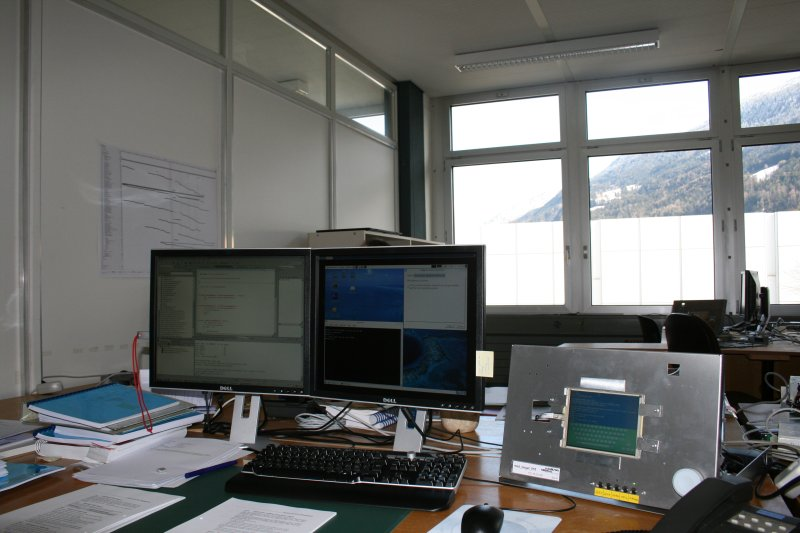
\includegraphics[width=\textwidth]{img/ham_pc_target.jpg}
    \end{minipage}}
 \caption{\label{My development environment PC and Power PC Target}
My development environment PC and Power PC Target}
\end{figure}

\subsubsection{PVCS}
PVCS is our control version manager, each project has its own PVCS database, the Nemo project uses it to store its Rhapsody Model, all the service scripts needed by the development team. It also contains the last project libraries, with the corresponding hardware BSP, and VxWorks image.
\\
Each PVCS files get a unique revision number when it is committed or added to the database, a common label can be given over different files, which permit to get the project on a precise state, only using the appropriate label.
\\
The PVCS program is both available under Graphical interface, and command line.

\subsubsection{EDO}
EDO is the intern document reference, all the produced documentation have to fit to the Hamilton-Medical pattern. EDO permits us to cross reference the different available documents, using Visual Basic Macro, EDO is powered by PVCS for the attribution of unique Numbers.
\\
Basically EDO is used to create and manage all the project documentation. We can share a document with other authors, finally when the document is up to date we release it in the system.
\\
Afterward some 'Korex' process permits us to correct add some details to a document. All this modification are definitively validated with a new revision. Some time a revision is preceded by some review meeting to ensure that the concerned people come to an agreement.

\subsection{Telelogic Rhapsody}
% parler de webify de state charts
Rhapsody is a industry's leading Model-Driven Development environment based on UML 2.0 that allows full application generation for our embedded software. Through Rhapsody's Model Driven Architecture (MDA) approach, we can rapidly target the platform independent application model to a real time embedded operating system. Rhapsody lends itself to an iterative design approach where our software can be constantly executed and validate on the host environment, then brought right down to the embedded target application, for target based testing.
\\
\\
Code that is generated from the model is just another view of the model, which allows the developer to make changes at the model or source level and have either dynamically reengineering. This dynamic model/code associatively gives our development team the flexibility to design at any level of granularity, and ensures that the model and documentation is consistent with the code.
\\
Our development team uses Telelogic Rhapsody to create the UML representation of the Nemo project. After having implemented the subsystem functionalities, Rhapsody generate the C++ source code for the selected operating system (VxWorks for PPC32). Finally this code is Compiled, and liked to a static library or an executable, depending of the subsystem goal.
\\
\\
Rhapsody provides some interesting features, like state charts design, where events permit to change from a state to another. The state charts diagram can be animated, which relieve the comprehension of the diagram to a visual angle.
\\
Another good feature is the possibility to interface the project through an http server (Webify), giving the possibility to perform some simulation with a simple html interface.
\\
\\
Rhapsody is a serious way to develop new embedded system, it use a powerful framework, which relay the complex implementation of part of the project to the Rhapsody Framework. It is simple to use, but the wide configuration properties make it too complex.

\subsection{WindRiver}

\subsubsection{VxWorks}
Wind River VxWorks platforms are the premier foundation for device software applications. The platforms are built on the industry-leading RTOS, VxWorks 6, and include tightly integrated middleware run-time technologies: networking, security, wireless, mobility, management, and graphics.
\\
VxWorks is the most established and widely deployed device software operating system. Its performance, scalability, and footprint make more than 300 million devices worldwide run faster and more reliably.
\\
\\
We have to distinguish two modes in WindRiver VxWorks systems, the kernel module and the real time process. Both have their advantages and drawbacks:\\

%TODO RTP: MCU KDM jungle direct access, slow down since verifications...
\begin{tabular}{|l|l|}
\hline
\multicolumn{2}{|c|}{VxWorks 6.x memory modes} \\
\hline
Kernel Module & Real Time Process \\ \hline
\hline
\end{tabular}

In the Nemo Project we use both of the modes, as RTP gives use more security about its memory management, it prevents from overwrite other part of allocated memory or worse, corrupt the system, many of the project libraries use this mode.
\\
But for critical modules which needs quick real time reaction like the Gas Delivery system, it is worth to use Kernel Module, its direct access to shared memory is a gain of time, but a rigorous coding is required.

%TODO explain the intern fonctionement of WindRiver, host shell target shell, WGD adgent, ...


\subsubsection{WindRiver Workbench}
Wind River Workbench is a collection of tools based on the Eclipse framework that permits building devices with Wind River Linux and VxWorks platforms. Workbench offers a open standards based suite for device software design, development, debugging, test, and management.
\\
The development phase is achieved by Rhapsody but for debugging complex program, WindRiver Workbench is from far more adapted. Basically the Wind River Debugger addresses the common and unique needs of developers involved with kernel
development, and application development.
\\
It incorporates the feature source-level debuggers, and target OS-aware development environments. Wind River provides the ability to debug complex environments and complex device software applications.
\\
Innovative multi-context debugging capabilities allow developers to debug code running in multiple contexts simultaneously. Multiple contexts mean any of the following:

\begin{itemize}
\item Multiple cores
\item Multiple tasks/processes/threads
\item Multiple processors types
\end{itemize}

Some other integrated tools are available with Workbench, Wind River ScopeTools are powerful and dynamic visualization tools for device software applications. They provide developers with visibility into the entire platform. You can monitor variables, optimize performance, and find memory problems everything while the system is still running.
\\
\\
Wind River MemScope ensures optimal use of memory which is a critical activity in device software design. Systems can run for days before failing due to non-characterized memory leaks.
\\
MemScope is an instant memory analyzer that provides greater visibility into memory usage.
\\
Wind River provides two compilers for developing with VxWorks 6.x: WindRiver Compiler(Diab) and Wind River GNU Compiler.
\\
\\
The VxWorks Host Shell, provides a command line interface that lets you download application modules and invoke both VxWorks 6.x and application modules subroutines. The Host Shell uses WDB agent to access the target through two connection types: network and serial.
\\
It also supports four interpreters C, CMD, Tcl, GDBmi, the Tcl interpreter is useful for starting process, it is employed to launch the Nemo Project.

%\newpage

\subsection{The development process}
% PVCS labels compilation of the code, launching of the project, ...
As the developer team have wrote code for a subsystem, they have to check that the modification they added did not badly affect the rest of the project.
\\
So they checkout the last revision of the project and compile it with their modified sources. After processing a successfully compilation and run the project, they commit their modifications into PVCS, attributing the 'current' label to their updated subsystem.

\begin{figure}[h]
\centering
  \framebox{
    \begin{minipage}{8cm}
     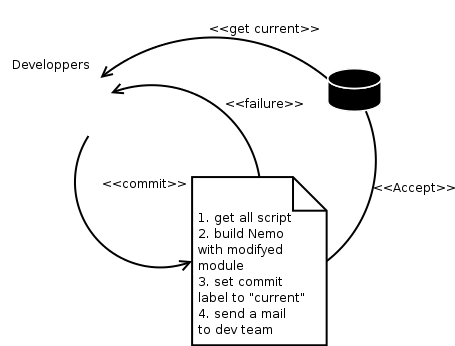
\includegraphics[width=\textwidth]{img/actual_workflow.png}
    \end{minipage}}
 \caption{\label{The Development workflow}
The Development workflow}
\end{figure}

The Nemo Project can be started by Windows batch script, launching a WDB server enabling the connexion between the host and the target. The executable .out or .vxe and the required module are transfered to the target. The main program is launched through a Tcl script.

\subsection{The Nemo Target}
Their are different prototype of the Nemo Target, one are featuring more components than others. The Traget I am working with contains the default hardware, a Power PC 603, with 128 Mo Ram, a touch screen, plus  Hardkeys fixed to the front pannel.
\\
The target I got on February had the first version of the hardware. But their are 3 other target having much more material, the blower an intern development, which delivers the required air pression. The flow sensors, permiting the measure of inspiration and expiration volumes, sound device for the alarming subsystem ... Depending on the part we are developing, we can borrow those target from other people of the Nemo team.
\\
\\
The next version of the Hardware is planned for end June, I developped a little program permitting to autoconfigure the target acessing to intern command of the MenMon BIOS. This programm was first written for testing on multiple Target containing different Hardware configuration but will also be used for updating massively the hardware.
\\
Finally this program was extended for updating a new firmware automatically, using a Telnet connection and no more the serial port as it was done previously.

%____________________________________
%
%____________________________________

\newpage

\section{Available Technologies}
Well as my subject concerned Software Testing, I had to document me about this subject. In fact the maneer we test our project at EPITA is just one part of the software testing conception, Black Box Testing. Testing software is a complicated task, that require some prerequisite. The following diagram sum up the different step of Software testing:

\begin{figure}[h]
\centering
  \framebox{
    \begin{minipage}{14cm}
     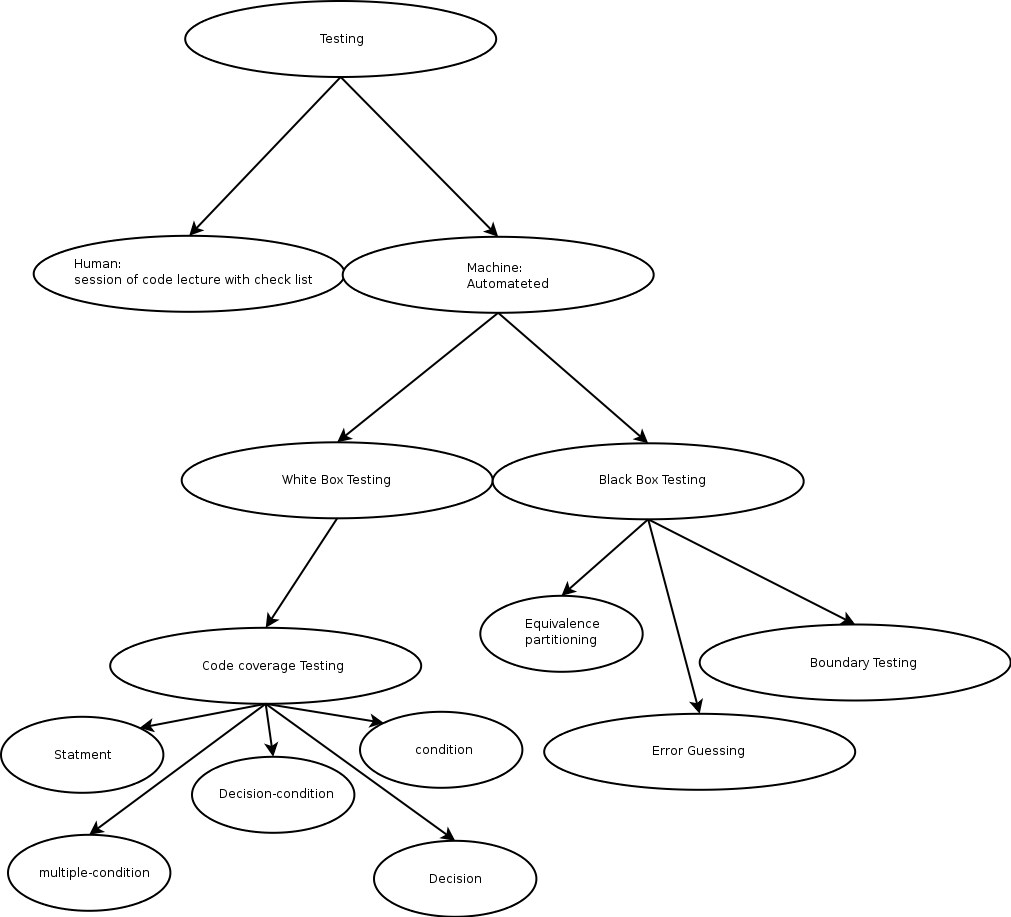
\includegraphics[width=\textwidth]{img/SoftTesting.png}
    \end{minipage}}
 \caption{\label{Software Test steps}
Software Test steps}
\end{figure}

I will give some more details in the next sections, about each part of this graph, so it will be easier to understand how I planned to test the Nemo project.

\subsection{Inspection and Walkthroughs}
There are both way to inspect a software project, in our case, Rhapsody produce some UML model, permitting us to discuss of the different choosen modelisation. Design walktrough are organised for detecting some basic missconception of the software. In the same manner, human can test the code their write, during code review. We spoke about human testing since this phase can not be automated.

\subsubsection{Code inspection}
% code inspection, an error checklist for code inspection % PCLINT
A code inspection is a set of procedures and error-detection techniques for group code reading. Most discussions of code inspections focus on the procedures.
\\
The team should be composed of 4 people, a moderator who is like a quality-control engineer. The second team
member is the programmer. The remaining team members usually are the s designer and a test specialist.

\subsubsection{Walkthroughs}
In a walkthrough, a group developers ofwith three or four being an number optimalperforms the review. Only one of the participants
is the author of the program. Therefore, the majority of program testing is conducted by people other than the author, which
follows the testing principle stating that an individual is usually ineffective in testing his or her own program.
\\
\\
For both Code inspection and walktrough, a good method is to collect the common errors type on a check list and analyse the code to prevent this kind of errors:

\begin{itemize}
\item Data Reference Errors
\item Data-Declaration Errors
\item Computation Errors
\item Comparison Errors
\item Control-Flow Errors
\item Interface Errors
\item Input/Output Errors
\end{itemize}

\subsubsection{DeskChecking}
A desk check can be viewed as a one-person inspection or walkthrough:
A person reads a program, checks it with respect to an error list, and walks test data through it.
\\
For most people, desk checking is relatively unproductive. One reason is that it is a completely undisciplined process.

\subsubsection{Peer Rating}
Peer rating is a technique of evaluating anonymous programs in terms of their overall quality, maintainability, extensibility, usability, and clarity.
The purpose of the technique is to provide programmer self-evaluation. This process improve the quality of the code, but does not test the software source code.

\subsection{Test Case Design}
The most important consideration in program testing is the design and creation of effective test cases.
Testing cannot guarantee the absence of all errors. Test-case design is so important because
complete testing is impossible; a test of any program must be necessarily incomplete. The obvious strategy, then, is to try to make tests
as complete as possible.
\\
\\
Let's introduce both White Box and Black Box testing methodologies. The recommended procedure is to develop test cases using the
black-box methods combined with white-box methods creating additional test cases.

\subsubsection{White Box}
White-box testing is concerned with the degree to which test cases exercise or cover the logic (source code) of the program. Let's detail the different coverage type we can aim.
% Statement coverage
\paragraph{Statement coverage}
It may seem that a worthy goal would be to execute every statement in the program at least once. Unfortunately, this is a weak criterion.
% Decision coverage
\paragraph{Decision coverage}
A stronger logic-coverage criterion is known as decision coverage or branch coverage. This criterion states that you must write enough test cases that each decision has a true and a false outcome at least once.
\\
Decision coverage requires that each decision have a true and a false outcome, and that each statement be executed at least once.

% Condition coverage
\paragraph{Condition coverage}
A criterion that is sometimes stronger than decision coverage is condition coverage.
In this case, you write enough test cases to ensure that each condition in a decision takes on all possible outcomes at least once.
It cause every individual condition in a decision to be executed with both outcomes.

% Decision-condition coverage
\paragraph{Decision-condition coverage}
Decision/condition coverage requires sufficient test cases that each condition in a decision takes on all possible outcomes at least once, each
decision takes on all possible outcomes at least once, and each point of entry is invoked at least once.

% Multiple-condition coverage
\paragraph{Multiple-condition coverage}
multiple-condition coverage requires that we write sufficient test cases that all possible combinations of condition outcomes in each decision, and all points of entry, are invoked at least once.

\subsubsection{Black Box}
Black box is technical jargon for a device or system or object when it is viewed primarily in terms of its input and output characteristics.

\paragraph{Equivalence partitioning}
Testing a program limits to trying a small subset of all possible inputs. wanting to select the right subset, the subset with the highest probability of finding the most errors.
\\
Each test case should invoke as many different input considerations as possible to minimize the total number of test cases necessary. After we can try to partition the input domain of a program into a finite number of equivalence classes such that we can reasonably assume that a test of a representative value of each class is equivalent to a test of any other value.

\paragraph{Boundary-value analysis}
Experience shows that test cases that explore boundary conditions have a higher probability to provoque errors than test cases that do not.
Boundary conditions are those situations directly on, above, and beneath the edges of input equivalence classes and output equivalence classes.

\paragraph{Error guessing}
Some poeple surmise, both by intuition and experience, certain probable types of errors and then write test cases to expose those errors.
The idea is to enumerate a list of possible errors or error-prone situations and then write test cases based on the list.
For instance, the presence of the value 0 in a s input is an error-prone situation.

\subsection{Module Testing}
Module testing (or unit testing) is a process of testing the individual subprograms, subroutines, or procedures in a program.
That is, rather than initially testing the program as a whole, testing is first focused on the smaller building blocks of the program.
\\
\\
Module testing is manages the combined elements of testing, since attention is focused initially on smaller units of the program. Second it eases the task of debugging, since, when an error is found, it is known to exist in a particular module.
Finally, module testing introduces parallelism into the program testing process by presenting us with the opportunity to test multiple modules simultaneously.

\subsubsection{Test Case Design}

Two types of information are needed when designing test cases for a module test:
\begin{itemize}
\item a specification for the module and the s source code.
\item The specification typically defines the s input and output parameters and its function.
\end{itemize}

\subsubsection{Incremental Testing}
%top down versus bottom up
In performing the process of module testing, there are two considerations:
\begin{itemize}
\item the design of an effective set of test cases, and the manner in which the modules are combined to form a working program.
\item The second consideration is important because it has implications for the form in which module test cases are written, the types of test tools that might be used, the order in which modules are coded and tested, the cost of generating test cases, and the cost of debugging.
\end{itemize}

Should we test a program by testing each module independently and then combining the modules to form the program, or should you combine the next module to be tested with the set of previously tested modules before it is tested? The first approach is called nonincremental bigbang testing or integration; the second approach is known as incremental testing or integration.
\\
\\
Two incremental approaches are available, top-down and bottom-up development or testing, both have their adventage and drawback.

\paragraph{Top-down}
Top-down testing represents a strategy of ordering the coding and testing of modules.
\\
The top-down strategy starts with the top, or initial, module in the program. After this, there is no single right procedure for selecting the next module to be incrementally tested.
\\
The only rule is that to be eligible to be the next module, at least one of the module��s subordinate (calling) modules must have been tested previously.

\paragraph{Bottum-up}
Bottom-up testing begins in a manner that is identical to a nonincremental test (i.e., when the bottom, or terminal, modules are tested), but bottom-up testing is an incremental strategy.
\\
The bottom-up strategy begins with the terminal modules in the program (the modules that do not call other modules).
\\
After these modules have been tested, again there is no best procedure for selecting the next module to be incrementally tested.
\\
The only rule is that, to be eligible to be the next module, all of the module��s subordinate modules (the modules it calls) must have been tested previously.
\newpage
\paragraph{Comparison}

Let's expose the advantages and drawback of both methodes\footnote{This charts are inspired from The Art of Software Testing}

\begin{itemize}
\item Top-down Testing:
\begin{figure}[ht]
\begin {center}
\begin{tabular} {|m{6cm}|m{6cm}|}
\hline
Advantages & Disadvantages \\
\hline
This is advantageous if major flaws occur toward the top of the program.& Stub modules must be produced.\\
\hline
Once the I/O functions are added, representation of test cases is easier. & Stub modules are often more complicated than they first appear to be.\\
\hline
Early skeletal program allows demonstrations and boosts morale. & Before the I/O functions are added, the representation of test cases in stubs can be difficult.\\
\hline
 & Test conditions may be impossible, or very difficult, to create.\\
\hline
 & Observation of test output is more difficult.\\
\hline
& It allows one to think that design and testing can be overlapped.\\
\hline
 & It induces one to defer completion of the testing of certain modules.\\
\hline
\end{tabular}
\end{center}
\end{figure}

\item Bottom-up Testing

\begin{figure}[ht]
\begin {center}
\begin{tabular} {|m{6cm}|m{6cm}|}
\hline
Advantages & Disadvantages \\
\hline
This is advantageous if major laws occur toward the bottom of the program. & Driver modules must be produced.\\
\hline
Test conditions are easier to create. & The program as an entity does not exist until the last module is added.\\
\hline
Observation of test results is easier & \\
\hline
\end{tabular}
\end{center}
\end{figure}
\end{itemize}

\subsection{System Testing}
Software development is largely a process of communicating information about the eventual program and translating this information from one form to another.
\\
For that reason, the vast majority of software errors can be attributed to breakdowns, mistakes, ... The purpose of System Testing is to avaoid these kind of errors. In the next sections we are dealing with different part of System Testing.

\subsubsection{Function Testing}
Function testing is a process of attempting to find discrepancies between the program and the external specification. An external specification is a precise description of the program's behavior from the point of view of the end user.
\\
\\
To perform a function test, the specification is analyzed to derive a set of test cases.
\\
The equivalence-partitioning, boundary-value analysis, and error-guessing methods are pertinent to function testing.
\\
The purpose of the function test is to expose errors and discrepancies with the specification, not to demonstrate that the program matches its external specification.

\subsubsection{System Testing}
System testing has a particular purpose: to compare the system or program to its original objectives.

\begin{itemize}
\item System testing is not limited to systems. System testing is the process of attempting to demonstrate how the program, as a whole, does not meet its objectives.
\item System testing, by definition, is impossible if there is no set of written, measurable objectives for the product.
\end{itemize}

The next figure illustrates why system testing is the most difficult testing process. The leftmost arrow in the figure, comparing the program to its objectives, is the central purpose of the system test, but there are no known test-case-design methodologies.
\\
The reason for this is that objectives state what a program should do and how well the program should do it, but they do not state the representation of the program's functions.


\begin{figure}[ht]
\centering
  \framebox{
    \begin{minipage}{10cm}
     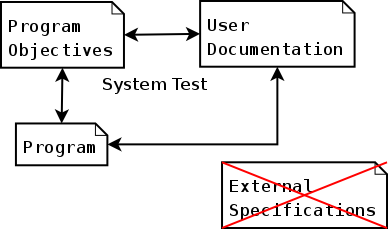
\includegraphics[width=\textwidth]{img/systemtest.png}
    \end{minipage}}
 \caption{\label{The system Test}
The system Test}
\end{figure}

In the following paragraphs more detail I especially explored for our project purpose.

\paragraph{Facility testing}

The most obvious type of system testing is the determination of whether each facility mentioned in the objectives was actually implemented.
\\
This type of testing often can be performed without a computer; a mental comparison of the objectives with the user documentation is sometimes sufficient.


\paragraph{Volume Testing}

Volume Testing is subjecting the program to heavy volumes of data. The purpose of volume testing is to show that the program cannot handle the volume of data specified in its objectives.

\paragraph{Stress Testing}
Stress testing subjects the program to heavy loads or stresses. In most of the cases, stress test describe a situation which should not occur, to see how the system react.
\\
Although many stress tests do represent conditions that the program likely will experience during its operation, other stress tests may truly represent ��never will occur�� situations.
\\
But this does not imply that these tests are not useful. If these impossible conditions detect errors, the test is valuable because it is likely that the same errors might also occur in realistic situations.

\paragraph{Usability Testing}
Today's software systems generally have undergone extensive human-factor studies,
here is a list of considerations:

\begin{itemize}
\item meaningful program output.
\item the error diagnostics (error message) are explicit and usefull (this program encountered a fatal error it will reboot windows like message have to be banned...)
\item easy to use program, knowing how to get to the main menu whyle navigating through several nenus or options menus
\end{itemize}

\paragraph{recovery testing}
Some recovery objectives that state how the system recovers from programming errors, hardware failures, and data errors.
\\
One objective of the system test is to show that these recovery functions do not work correctly. Programming errors can be purposely injected into a system to determine whether it can recover from them.
\\
\\
Hardware failures such as memory parity errors or I/O device errors can be simulated. Data errors such as noise on a communications line or an invalid pointer in a database can be created or simulated to analyze the system's reaction.

\subsection{Completion crieteria}
% when do we stop testing
One of the most difficult questions to answer when testing a program is determining when to stop. There is no way of knowing if the error just detected is the last remaining error.
\\
In fact, it is unreasonable to expect that all errors will eventually be detected. Knowing this statment, some methode can be applyed to for determine weather we should continue to test or not.
\\
\\
One problem is determining how to obtain the number of errors to be detected. Obtaining this number requires the following three estimates:
\\
\begin{itemize}
\item An estimate of the total number of errors in the program.
\item An estimate of what percentage of these errors can feasibly be found through testing.
\item An estimate of what fraction of the errors originated in particular design processes, and during what testing phases these errors are likely to be detected.
\end{itemize}

One method is to obtain them through experience with previous programs. Some of these require to be testing the program for some period of time,
record the elapsed times between the detection of successive errors, and insert these times into parameters in a formula.
\\

\newpage
\subsection{Development and Testing Processes}

\begin{figure}[ht]
\centering
  \framebox{
    \begin{minipage}{8cm}
     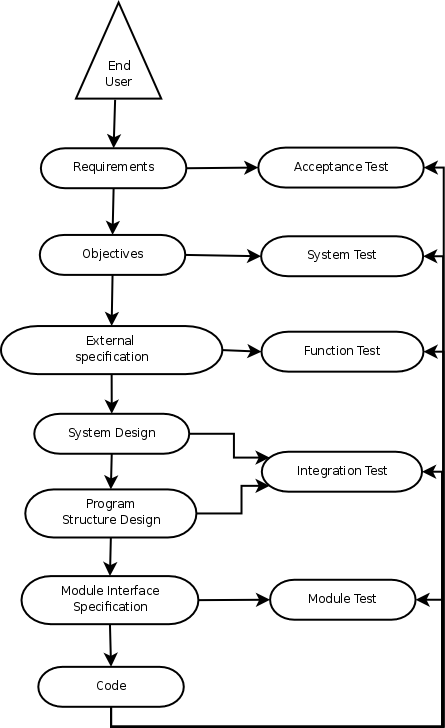
\includegraphics[width=\textwidth]{img/devandtest.png}
    \end{minipage}}
 \caption{\label{The correspondence between development and testing processes.}
The correspondence between development and testing processes.}
\end{figure}

A one-to-one correspondence between development and testing processescan be defined:

\begin{itemize}
\item The purpose of a module test is to find discrepancies between the program��s modules and their interface specifications.
\item The purpose of a function test is to show that a program does not match its external specifications.
\item The purpose of a system test is to show that the product is inconsistent with its original objectives.
\end{itemize}

% ce que j'ai du choisir d'utiliser pour effectuer mon projet
%vous detaillerez le panel des techniques et solutions possibles pour effectuer votre stage au regard de la problematique qui vous a ete assigner.

% code coverage
% multi threading process
% state charts testing / state machine testing
% test report

\subsection{Rhapsody Test Conductor}

Telelogic Rhapsody TestConductor is the first UML(Unified Modelling Language) compliant, scenario based test generation and validation suite for real-time embedded applications. With Rhapsody TestConductor developers can test their design against its requirements, throughout the development process, detecting design errors early on in the development process.
\\
\\
Rhapsody TestConductor enables users to check a design against its requirements, which have been captured as scenarios in a sequence diagram. These include system level requirements and derived requirements or scenarios that are defined by testing.
\\
When defining a system test, users can instantiate as many copies as needed for these sequences, effectively using them as test patterns.
\\
\\
Each instance of a sequence diagram can be defined as a monitor, in which case it silently observes and checks the behaviour of the design, warning of potential errors as the design evolves. Additionally, each instance of a sequence diagram can be defined as a test driver.
\\
Rhapsody TestConductor generates all of the messages that are emanating from the system border, while monitoring all other interactions that are defined in the Sequence Diagram as the design executes.

\subsection{Rhapsody Automatic Test Generator}
Rhapsody ATG allows users to define and test individual components for specific purposes such as State and Transition coverage, MC/DC coverage, or isolation of a particular class from the overall design. Additionally, ATG allows the user to identify model elements that have not been covered allowing for the identification of dead code at critically early stages of development. While test cases can be used for Unit Testing, Integration Testing, and Regression Testing.

\subsection{WindRiver Unit Tester}

Unit testing and integration testing are the lowest levels of testing performed during software development, where individual functions, classes, or subsystems of software are tested in isolation from other parts of a program. This level of testing is also the least expensive time to fix software bugs if they can be identified. Workbench Unit Tester is a plug-in that allows developers to more efficiently complete unit testing, integration testing, and code coverage analysis on the tests.
\\
\\
Unit Tester makes it easier for developers to perform unit testing as each function or class is written, thereby catching bugs earlier in the development process.
\\
Integrated coverage analysis provides statement, decision, MC/DC, entry point, and call-return metrics.
\\
\\
Unit Tester generates unit and integration tests in C or C++ code, so developers will not need to learn a special test language or commands.
\\
\\
This table will give you some comparison between the two tools I evaluated:

\begin{figure}[h]
\centering
  \framebox{
    \begin{minipage}{12cm}
     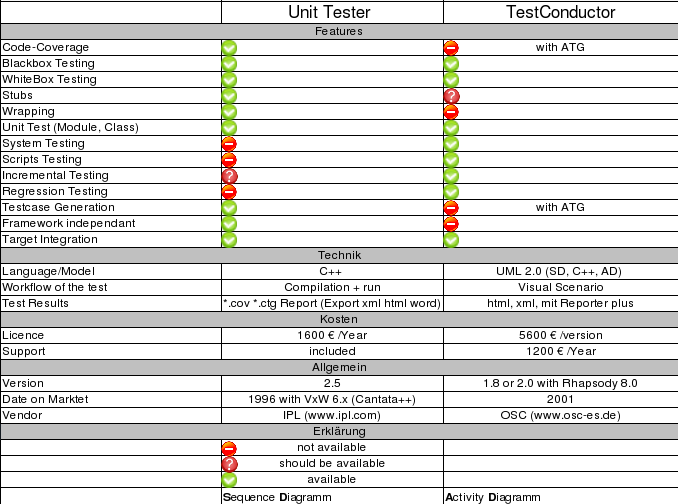
\includegraphics[width=\textwidth]{img/toolcompare.png}
    \end{minipage}}
 \caption{\label{Test tools comparisons}
Test tools comparisons}
\end{figure}

\subsection{Rhapsody - Workbench integration}
The Nemo Project is the first project of \emph{Hamilton-Medical}, developping the Software with Rhapsody tool base on WindRiver OS: VxWorks 6.3.
\\
Both tools have their own process (makefiles...), that are completly different. But we have to make some bridge between those Tools, for working efficienly. Well tree possibilities are available, but only two of them are concretly usable:


\subsubsection{Workbench Managed Makefiles} is the basic solution proposed by WindRiver, since it analyses the project options and source code and generate the corespoding makefile.
\subsubsection{Eclipse plugin} Rhapsody founrnish an Eclipse Plugin to link its Project to a Workench project, Basically it write a additional Makefile included by the managed build makefile of Workbench, permitting to compile the project under Workbench.
\subsubsection{Adapting Rhapsody Makefile} and use it as user defined Makefile in the Workbench project.
\\
\\
The first solution rather needs a lot of hand work, including libraries, one more time, setting the include path one more time. The two other solution give more perspectives.

\subsection{Linux}
One of the possibility of automation of the test process was by using a linux server for performing multiple test tasks.
Currently their is no Computer powered by a Linux System, and few People have Linux Know How. Well I developped some example to give some concrete point of view about Linux.
\\
First I installed a VmWare Virtual Machine manager, and used a Ubuntu Linux to perform the Demo. I also profited to install the trac deamon, and a personal svn used for making revision of my working documents.
\\
\\
Finally Ulrich and I did some comparison between the scripting possibilities offered by a Linux and Windows OS for the Nemo Project.
\\
The goal of this comparison was to emphasis the automation possibility of testing on both Operating Systems.

\begin{figure}[ht]
\begin {center}
\begin{tabular} {|m{6cm}|m{6cm}|}
\hline
Linux & Windows \\
\hline
Tcl and Tk (GUI) are originally integrated to the system. & Windows required to install it\\
\hline
Terminal shell include powerfull built-in commands permitting to directly handle serial flow. & under Windows, Hyperterminal are not free 75\$ for the licence\\
\hline
unchanged stable command shell for years & Windows Batch command shell is still very limited \\
\hline
Procedural scripting language are by default available perl, sh, ruby, ... & Under Windows, Batch is the default scripting language, but Perl and other scripting language can also be installed\\
\hline
\end{tabular}
\end{center}
\end{figure}

\subsection{Software Testing Workflow}
As I integrated the Nemo project, the Software Testing Workflow did not exist. I fortunaltly got every information concerning the G5 Project test process. The G5 project had some special status since they had some test case which came from Cantata++ tool, predecessor of the Workbench Unit Tester. So one of their work consisted to adapt theses test cases.
\\
\\
I also was granted the access to the G5 PVCS, which formed a large unit Tester database. But the G5 Project was developed in C language, that made the test situation quite different. But I inspired me from some process directly toutching Unit Tester.
\\
\\
G5 project uses multiple batch script for applying their Testing Workflow, using one unit Tester source code template to pattern new test cases, and compile the test project with unit Tester.
\\
As soon as these Batch script contain hundreads of line, the readability is affected, due to the non procedurale scripting language. Starting the compiled project is done with help of Tcl scripts, directly interpreted by the host shell fournished by WindRiver.
\\
\\
The choice had to be made on the script language we want to use for support the Nemo Project Test Workflow.

\subsection{Project compilation}
Both Tools Rhapsody and WindRiver provides some different build process through diffrent Makefiles. The Rhapsody Makefile is readable whereas the WindRiver makefile is generated, dense and hard to edit.
\\
Two possibilities were envisageable:
\begin{itemize}
\item compile the project calling the makefile one after another with several batch files (currently used).
\item compile the project with a toplevel makefile, calling recursive submakefile of the different sub directories.
\end{itemize}

Well what is the difference?! In fact in the first solution, employes the Makefile pocess like the second solution. But the main difference using the second method is that we are profiting of the power of GNU Makefile that only Build/Rebuild the neceassary part of the project. This selective compilation is for the moment not used, every build of the Nemo project is in fact a complete rebuild of the project.

\subsection{Wiki}
As explained in the previous sections, the Nemo project is developed under Microsoft Windows, the communication means are concentrate arround Microsoft outlook. Unfortunatelly the Nemo Know how can get lost, their is no common ressource where people can freely add their notice about how to solve a problem. The only offered solution is to copy the mail communication to a common folder.
\\
\\
So I proposed some alternative solution, a Wiki based on the trac engine \url{http://trac.edgewall.org/} we sucessfully used the same tool for our project managment at EPITA (GISTR). The Wiki concept is to share information very easilly, on a web page. Every user can contribuate by editing the Wiki.
\\
Well I presented the Wiki feature to the Nemo team which was for the majority enthousiastic about the idea. For the moment the Wiki is regullaly edited by Ulrich and me, now it has several sections that contain usefull information about the project and the tools we use. We still reference the EDO documents which stay the official document, but we also reference to the Wiki in EDO documents.
\\
The Goal is to install the wiki on a Linux Server, maybe make one wiki per project, the support would be assured by Valentin Conrad, unique Person using a Linux based computer at work.

\newpage
\section{Chosen solutions}
%Dans ce chapitre, vous affirmerez puis justifierez vos choix/votre solution en mentionnant pourquoi les alternatives se sont reveles inadaptees. L'utilisation d'une grille de notation multicriteres sera apprecier. les appreciations subjectives sertont a eviter

\subsection{Test Workflow}

\begin{figure}[h]
\centering
  \framebox{
    \begin{minipage}{15cm}
     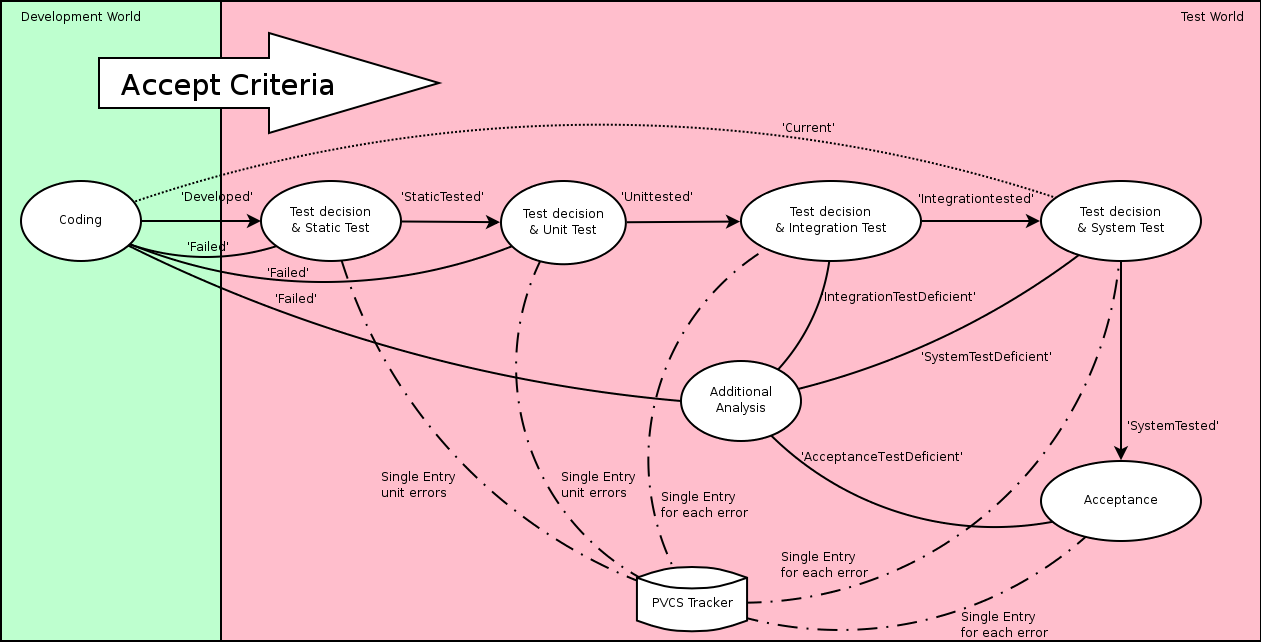
\includegraphics[width=\textwidth]{img/TestWorkflow.png}
    \end{minipage}}
 \caption{\label{Test Workflow}
Test Workflow}
\end{figure}


\subsection{Rhapsody - Workbench integration}

\begin{figure}[h]
\centering
  \framebox{
    \begin{minipage}{15cm}
     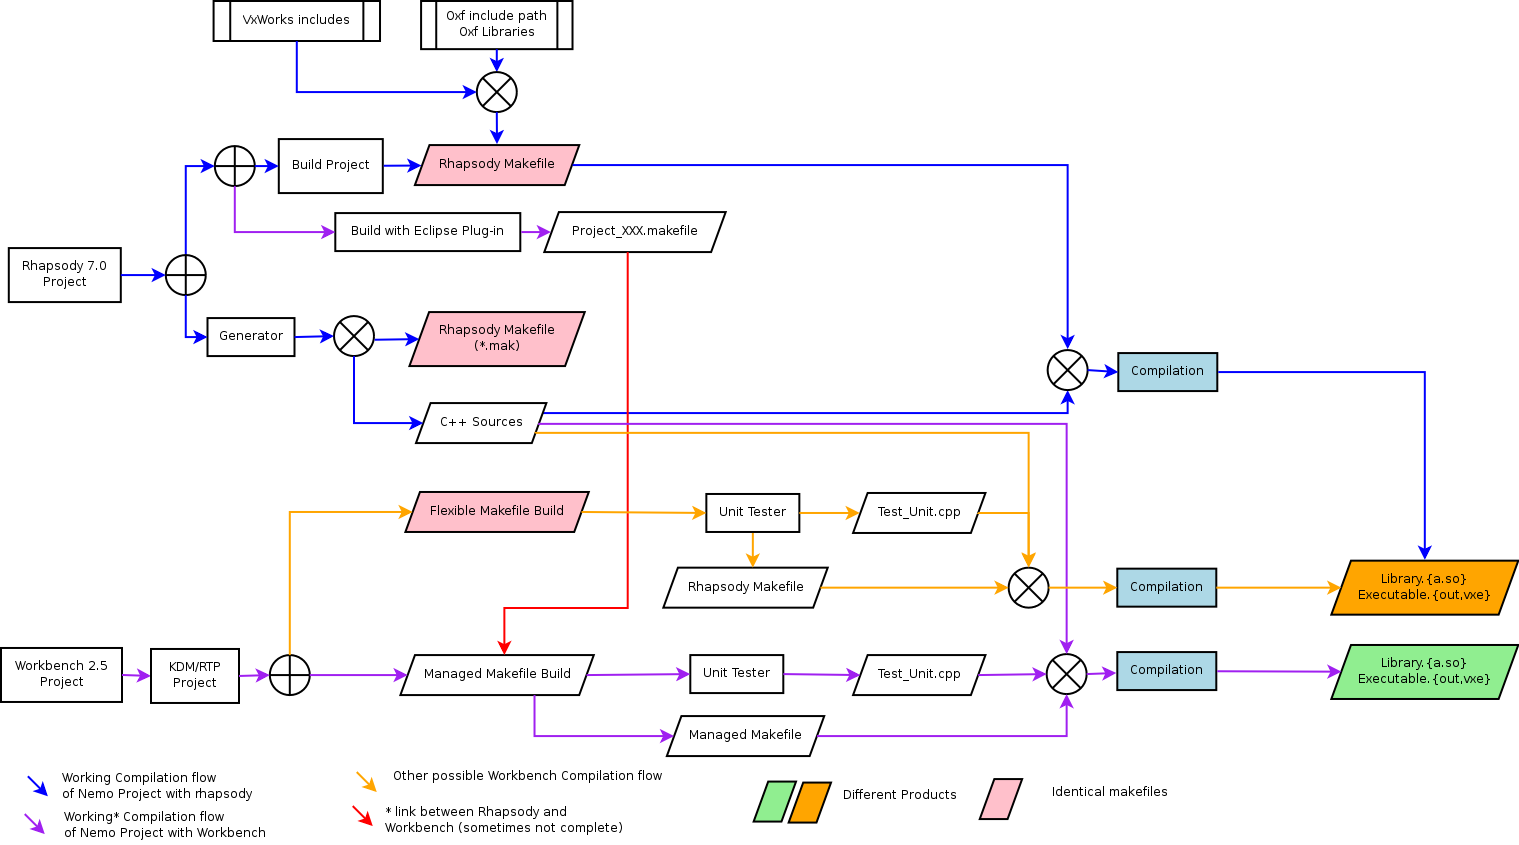
\includegraphics[width=\textwidth]{img/Rhapsody-Workbench.png}
    \end{minipage}}
 \caption{\label{Rhapsody Workbench Integration}
Rhapsody Workbench Integration}
\end{figure}

\subsection{WindRiver Unit Tester}

\subsection{Perl scripting}

\begin{figure}[h]
\centering
  \framebox{
    \begin{minipage}{12cm}
     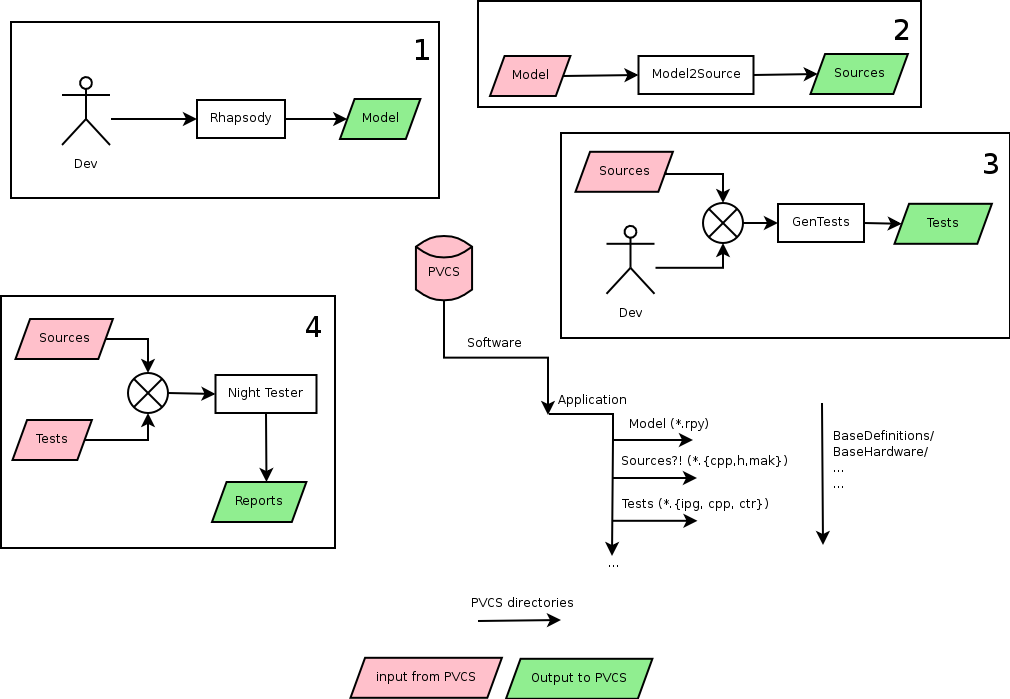
\includegraphics[width=\textwidth]{img/PVCS_2_Test.png}
    \end{minipage}}
 \caption{\label{Test Workflow}
Test scripts using PVCS}
\end{figure}


\newpage
\section{Encountered problems}
% vous preceiserez les problemes auxquels vous avez fait face et en quoi ils ont oriente, confirme, modifie les choix de votre solution.

\subsection{Interaction of Rhapsody - Workbench}
\subsubsection{obtaining the same building process}
\subsubsection{lacking documentation on the eclipse plug-in}
\subsubsection{Rhapsody framework}

\subsection{WindRiver Unit Tester}
\subsubsection{Test automation}
\subsubsection{Lacking Documentation}
\subsubsection{Flexible build}

\subsection{Submit Process}
\subsubsection{PVCS Labels}
\subsubsection{Development - test Process}


\newpage
%----------------------------------------------------------------------------------------------------------------------------------------------------------
\chapter{Conclusion}%_________________________________________________~10 pages
%le but de ce chapitre est de permettre au jury de mesurer la valeur ajoutee que vous avez apporte a l'entreprise et de comprendre en quoi vous avez repondu au besoin de l'entreprise.

\section{Internship interest for Hamilton}
% vous detaillerez l'interet a court et long terme du stage pour l'entreprise, les perspectives ouverte par le sujet.
% test team, using the test concept for the next project
% reusability of the code and test cases

\section{Personal opinion about the internship}
%vous detaillerez l'interet personnel et ou organisationnel aquis pendant le stage.
% - stage interessant sur un sujet que nous n'avions pas detailler a l'epita...
% - aquisition de se coller aux normes, ainsi que de travailler sur un projet qui exige une qualite superieur
% - quelques notions de medecine
% - perfectionement de mon allemand
% - emauche CDI :P
% - Approfondissement des outils windriver et Rhapsody
% - Application direct de la modelisation embaquer
% - tester une application avec des containtes temps reeles.
% - liens avec les autres services, hardware qualite


\section{The Hamilton Experience, improvements}
Industry analysts have determined that, when developing new products, testing consumes 70\% of development time and 50\% of the development costs.
With increasing pressure to deliver higher quality products in shorter time frames and with fewer resources, managers and developers
must continually evaluate the effectiveness of their testing process.

% testing earlier, extrem programing, apply for each conception of the dev the testing bijection, schema dev+test from the art of software testing
% give the oportunity to build a test team so that dev should not test their own code.
% test organisation, step by step, using gantt dia + charts of detected errors per week, test acomplishment, stat

% establish a comment norm doxygen or other with rhapsody.

% create test team meeting
% have a defined gantt timeline


\subsection{Performing the Tests}

One of the most vital considerations in implementing the tests is determining who should do it. Programmers shouldn't perform tests, neither should the organization responsible for developing the programs .

\subsection{Test Planning and Control}\index{Planning}

Considering that testing a large system could entail writing, executing, and verifying tens of thousands of test cases, handling hundread of classes, repairing thousands of errors, we are facing an immense project management challenge in planning, monitoring, and controlling the testing process.
\\
\\
An obvious mistake is that the planned resources (people, calendar time, and computer time) will be grossly underestimated. It is a notorious problem in the computing industry. The fact that the testing process falls at the end of the development cycle, meaning that resource changes are difficult.
\\
\\
The plan is the crucial part of the management of the testing process. Here is a list of improvment that could be applyed to the next \emph{Hamilton-Medical} project\cite{Glenford-04}: %TODO ref to The art of software testing

\begin{description}
\item [Objectives] The objectives of each testing phase must be defined.
\item [Completion criteria] Criteria must be designed to specify when each testing phase will be judged to be complete.
\item [Schedules] Calendar time schedules are needed for each phase. They should indicate when test cases will be designed, written, and executed.
\item [Responsibilities] For each phase, the people who will design, write, execute, and verify test cases, and the people who will repair discovered errors, should be identified. An arbitrator should be identified.
\item [Computer time] This is a plan for the amount of computer time needed for each testing phase (especially for compilation time).
\item [Hardware configuration] If special hardware configurations or devices are needed, a plan is required that describes the requirements, how they will be met, and when they are needed.
\end{description}

\newpage
%----------------------------------------------------------------------------------------------------------------------------------------------------------
\section*{Special Thanks}
In this section I would like to thank all the People who contribuated to my success for this Internship at \emph{Hamilton-Medical}:
\begin{itemize}
\item The Nemo Team
\item Roger Altermatt, my internship supervisor, for his patience and calm, leading the Nemo project.
\item Andreas Andreeg, Nemo Software Guru, for his precious advices.
\item Urs Reidt, New Products Responsible, for his clairvoyance for solving problem, choosing the best solution.
\item Ulrich Hauser, for his support, helping me taking crutial decision.
\item Romain Bornet, from NetModule Technical support.
\item Gion Durish, WindRiver Licence Responsible
\item Christian Frehner, responsible of G5 Unit Tester.
\item Cornelia ??? %TODO
\item Ralph Trauber
\item Dominik Novotni
\item Lars Schmohl
\item Joseph Brunner
\item Ricardo Lopez
\item Sandro Dalavalle
\item Katrin Schmitt from Human resources, especially for finding me a flat in Chur :)
\item Cecile Juon
\end{itemize}

Special thanks to Sara, for the time I procrastinate in her company ;)

\newpage
\appendix
\addcontentsline{toc}{chapter}{Bibliography}
\bibliographystyle{plain}
\bibliography{keller_e-report}

\addcontentsline{toc}{chapter}{Glossaire}
\printglosstex[1]
\addcontentsline{toc}{chapter}{Index}
\printindex

%bibliography
% the art of software testing
% Ralph Tauber hm future presentation
% H=MC^2 for the history part
% opportunities Dr. Adrian Frutiger

\newpage
\end{document}
